% Saved into the git report.tex at 2017/12/15 at 00:11 from this web
\documentclass[a4paper]{article}
\usepackage[utf8]{inputenc}
%\usepackage{pythonhighlight}

\usepackage{graphicx}
\graphicspath{{fig/}}
\usepackage{listings}
\usepackage{color}
\usepackage{float}

% Click on references
\usepackage{hyperref}

% Use better tables
\usepackage{booktabs}

% Units
\usepackage{siunitx}

\usepackage{minted}
\newminted{py}{%
%		linenos,
		fontsize=\footnotesize,
		tabsize=4,
		mathescape,
}
\newminted{text}{%
%		linenos,
		fontsize=\small,
		tabsize=2,
		mathescape,
}

\title{Lab 6 - CSN: Network dynamics}
\author{Pierre-Antoine Porte \\ \texttt{porte.pierreantoine@gmail.com}
\and Rodrigo Arias Mallo \\ \texttt{rodarima@gmail.com}}
\date{\today}

%%% \def\arraystretch{1.5}

\begin{document}

\maketitle

\section{Introduction}
%
In this session, we are going to generate some data by using 3 different 
variations of the dynamical principles in Barabasi-Albert models (BA models in 
the future).  Those principles are: vertex growth and preferential attachment.  
The different variations of models we will implements are:
%
\begin{itemize}
	\item \textbf{A}: Vertex growth and preferential attachment (original).
	\item \textbf{B}: Vertex growth and uniform random attachment.
	\item \textbf{C}: Suppressed growth and preferential attachment.
\end{itemize}
%
Those generator models were simulated and the stored data will let us to analyze 
mathematical properties. In this report we will show, discuss and explain the 
results as well as the details of the implementation.
%
\section{Results}
%
For each generation model (A, B and C), two metrics are analyzed, the 
distribution of the degrees of the nodes (D), and the evolution of a node as the 
graph grows over time (T).  We track the evolution of 4 different nodes selected 
from different points in the simulation. In the figures from~\ref{fig:all_dd_A} 
to~\ref{fig:bestC_dt1000} the best models are plotted along with the data. The 
notation for each model has been slightly changed, to avoid confusion. All 
models from session 2 where renamed with a T as prefix, and those from the 
session 3 a D as prefix instead. Those prefixes let us distinguish between say 
the model $D1$ and $T1$, as one is modeling the degree distribution, and the 
other the degree over time. The models for the evolution of degree over time can 
be shown in table~\ref{tab:Tmodels}, the models for the degree distribution are 
used in the minimum log likelihood form, and the only change is $\gamma = 3 $ in 
model 2 (see table 2 of session 2).
%
The tables~\ref{tab:AICdd} to~\ref{tab:AICdt1000} use AIC to
measure $\Delta = AIC - AIC_{best}$ of each model.
%
\begin{table}[H]
	\centering
	\begin{tabular}{cll}
		\toprule
		Model & Function & Parameters\\
		\midrule
		T0  & $f(n) = at$								& $a$ \\
		T1  & $f(t) = (t/2)^b$					& $b$ \\
		T2  & $f(t) = at^b$ 						& $a,b$\\
		T3  & $f(t) = ae^{ct}$					& $a,c$\\
		T4  & $f(t) = a\log t$					& $a$\\
		T5  & $f(t) = at^be^{ct}$				& $a,b,c$\\
		T1+ & $f(t) = (t/2)^b + d$			& $b,d$\\
		T2+ & $f(t) = at^b + d$					& $a,b,d$\\
		T3+ & $f(t) = ae^{ct} + d$			& $a,c,d$\\
		T4+ & $f(t) = a\log t + d$			& $a,d$\\
		T5+ & $f(t) = at^be^{ct} + d$	& $a,b,c,d$\\
		\bottomrule
	\end{tabular}
	\caption{The list of models to fit the degree over time.}
	\label{tab:Tmodels}
\end{table}

\newpage

\begin{figure}[H]
		\centering
		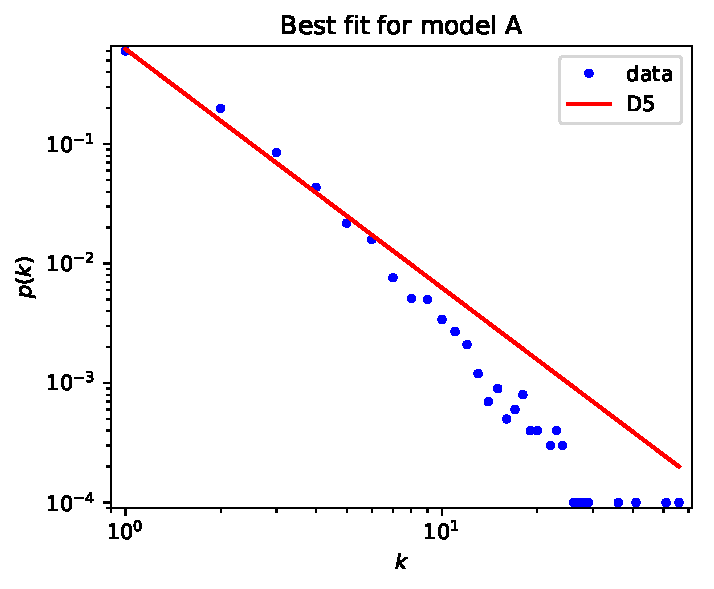
\includegraphics[width=0.5\textwidth]{modelA/best_dd.pdf}
		\caption{Distribution degree for model A}
		\label{fig:all_dd_A}
\end{figure}
%
\begin{figure}[H]
		\centering
		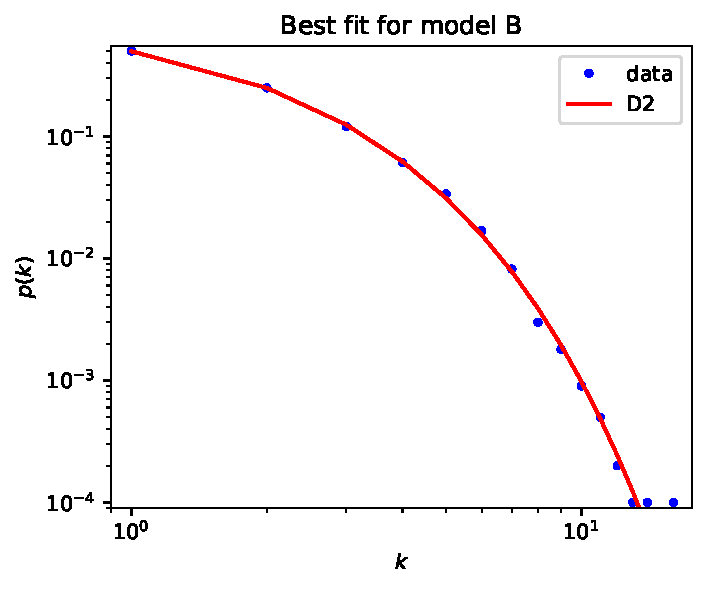
\includegraphics[width=0.5\textwidth]{modelB/best_dd.pdf}
		\caption{Distribution degree for model B}
		\label{fig:all_dd_B}
\end{figure}
%
\begin{figure}[H]
		\centering
		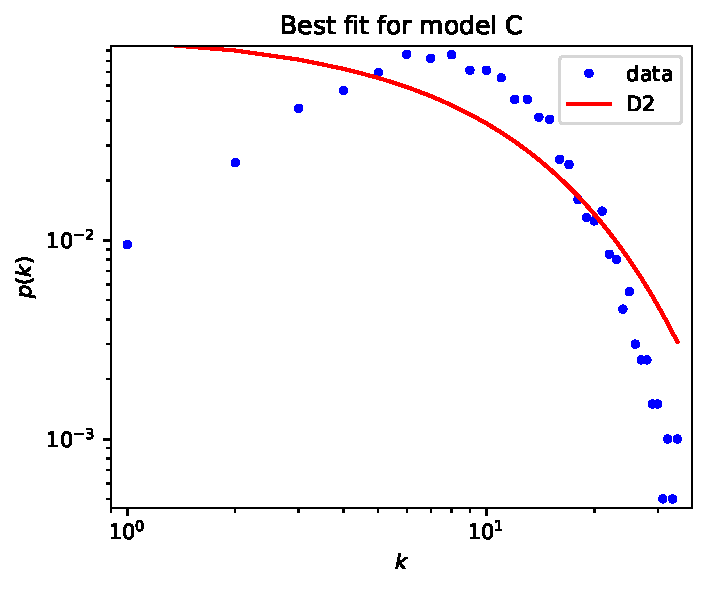
\includegraphics[width=0.5\textwidth]{modelC/best_dd.pdf}
		\caption{Distribution degree for model C}
		\label{fig:all_dd_C}
\end{figure}
%
\begin{figure}[H]
    \centering
		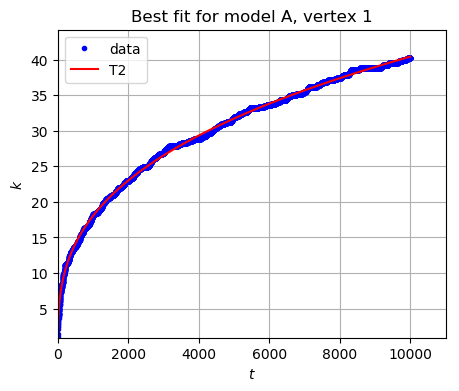
\includegraphics[width=0.5\textwidth]{modelA/best_dt1.png}
		\caption{Degree over time for model A with vertex at $t=1$}
%		\label{fig:all_dd_C}
\end{figure}
%
\begin{figure}[H]
    \centering
		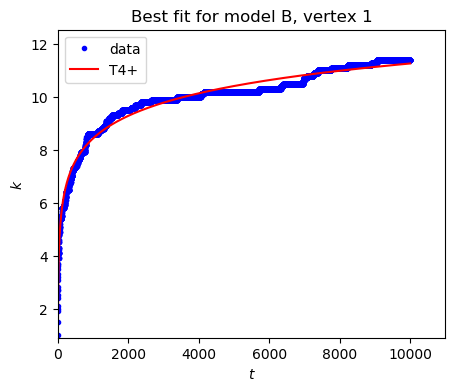
\includegraphics[width=0.5\textwidth]{modelB/best_dt1.png}
		\caption{Degree over time for model B with vertex at $t=1$}
%		\label{fig:all_dd_C}
\end{figure}
%
\begin{figure}[H]
		\centering
		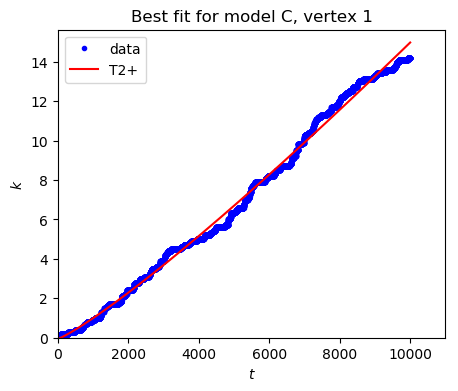
\includegraphics[width=0.5\textwidth]{modelC/best_dt1.png}
		\caption{Degree over time for model C with vertex at $t=1$}
%    \label{fig:all_dd_C}
\end{figure}
%
\begin{figure}[H]
    \centering
		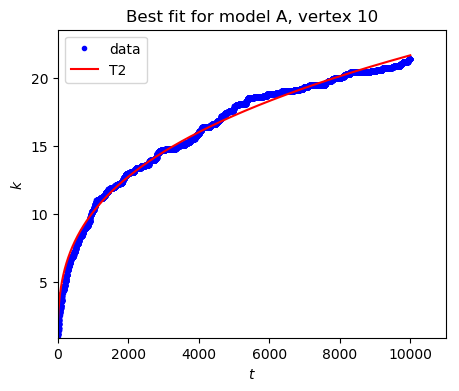
\includegraphics[width=0.5\textwidth]{modelA/best_dt10.png}
		\caption{Degree over time for model A with vertex at $t=10$}
%		\label{fig:all_dd_C}
\end{figure}
%
\begin{figure}[H]
    \centering
		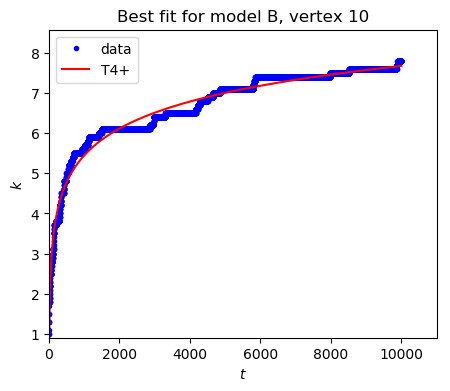
\includegraphics[width=0.5\textwidth]{modelB/best_dt10.png}
		\caption{Degree over time for model B with vertex at $t=10$}
%		\label{fig:all_dd_C}
\end{figure}
%
\begin{figure}[H]
		\centering
		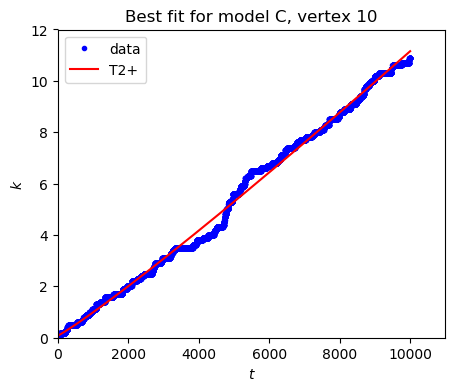
\includegraphics[width=0.5\textwidth]{modelC/best_dt10.png}
		\caption{Degree over time for model C with vertex at $t=10$}
%		\label{fig:all_dd_C}
\end{figure}
%
\begin{figure}[H]
    \centering
		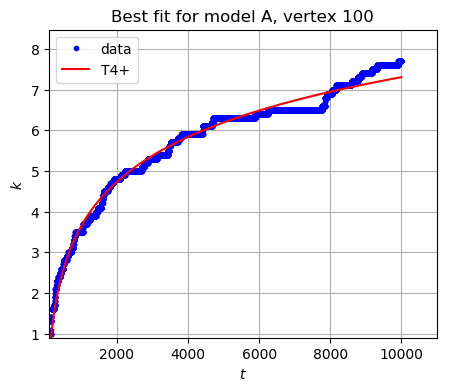
\includegraphics[width=0.5\textwidth]{modelA/best_dt100.png}
		\caption{Degree over time for model A with vertex at $t=100$}
%    \label{fig:all_dd_C}
\end{figure}
%
\begin{figure}[H]
    \centering
		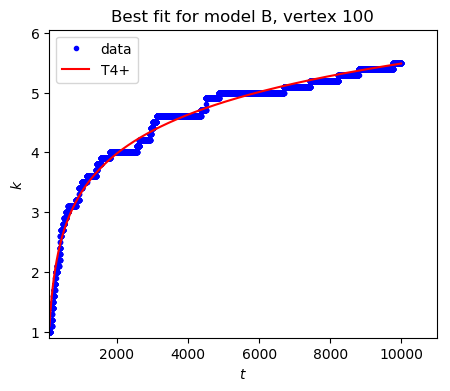
\includegraphics[width=0.5\textwidth]{modelB/best_dt100.png}
		\caption{Degree over time for model B with vertex at $t=100$}
%    \label{fig:all_dd_C}
\end{figure}
%
\begin{figure}[H]
		\centering
		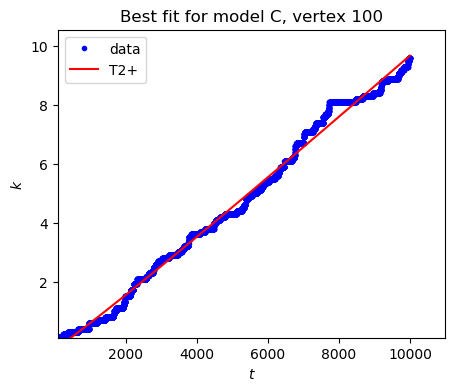
\includegraphics[width=0.5\textwidth]{modelC/best_dt100.png}
		\caption{Degree over time for model C with vertex at $t=100$}
%    \label{fig:all_dd_C}
\end{figure}
%
\begin{figure}[H]
    \centering
		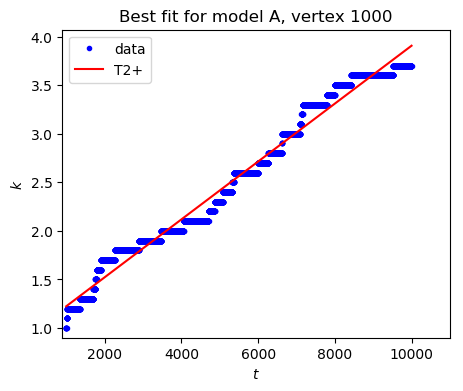
\includegraphics[width=0.5\textwidth]{modelA/best_dt1000.png}
		\caption{Degree over time for model A with vertex at $t=10000$}
%		\label{fig:all_dd_C}
\end{figure}
%
\begin{figure}[H]
    \centering
		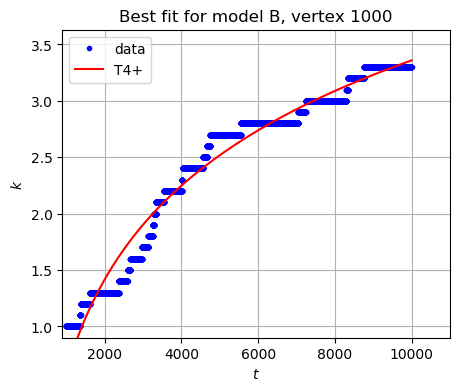
\includegraphics[width=0.5\textwidth]{modelB/best_dt1000.png}
		\caption{Degree over time for model B with vertex at $t=1000$}
%    \label{fig:all_dd_C}
\end{figure}
%
\begin{figure}[H]
		\centering
		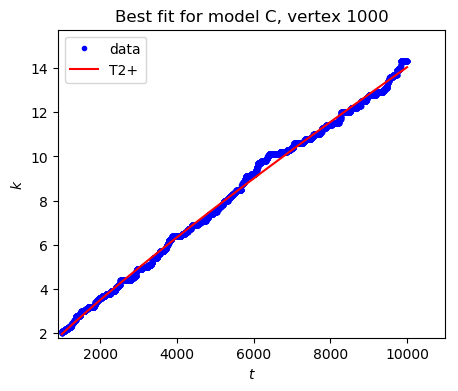
\includegraphics[width=0.5\textwidth]{modelC/best_dt1000.png}
		\caption{Degree over time for model C with vertex at $t=1000$}
		\label{fig:bestC_dt1000}
\end{figure}

%
% TODO: add dt1->1000 for each model
%
\section{Discussion}

We used $m_0$ and $n_0$ always with the same values (which can be however 
different for each model). We never compared the models with different $m_0$ or 
$n_0$ for the same model. It could have indicate us if the model behave 
differently given different graph in input. We could have went further and do 
this but we preferred to focus on the analysis of our different models with the 
input specified in the methods section.

\subsection{Model A}

% TODO Understand why we don't have this barabasi albert property %

\paragraph{Vertex degree over time}

We checked if the power-law dependency with 1/2 exponent gives the best fit to 
all the time series as required by the statement. This power-law dependency is 
not the best fit. This power-law is model T1, which has an AIC higher than model 
T2 (see tables \ref{tab:AICdt1} to \ref{tab:AICdt1000}). In fact the best model 
is model T2, defined as $f(t) = at^b$, which is the exponential growth. It makes 
sense because with one free parameter we can better optimize this model to fit 
the data, by adapting $b$ to somewhat close to 1/2 as expected in model T1, 
however we may be overestimating the data.
%
If we look at table \ref{tab:paramsdt1} to \ref{tab:paramsdt1000}, we
see that $b \approx 0.5$ only for $t_i = 1000$ (table \ref{tab:paramsdt1000}).

%\subsection{Degree distribution}

\subsection{Model B}

\paragraph{Vertex degree over time}

For table \ref{tab:AICdt1} to \ref{tab:AICdt1000}, best model is as suggested by 
the statement, the logarithmic model T4. Indeed, we have 0 as $\Delta$ for the 
vertex degree over time for this model and for every $t_i$ chosen to look at the 
vertex.

%todo add plot

\paragraph{Degree distribution}


The best model for the degree distribution for the Barabasi Albert model without
preferential attachment is the geometric one (model D1). Actually only the
variant of the geometric model is good (model D1+), as we can see in table
\ref{tab:AICdd}. The model D1 has a $\Delta$ too high. However by replacing
correctly the generated data from model D1, we now have a $\Delta$ of 0.
Thus, the geometric model variant is the best model.

%By looking at the figure \ref{fig:ADD THE PLOT}, we can clearly see that
%the geometric model (orange one) is a really good approximation of our data. It 
%even goes through a lot of points of the actual data point we have.

%todo add ref plot


\subsection{Model C}

\paragraph{Vertex degree over time}

As expected by statement, the degree over time should fit a linear scale. By 
computing the AIC and making the $\Delta$ (see tables \ref{tab:AICdt1} to 
\ref{tab:AICdt1000}) we have seen that the linear model was good. Also, we are 
really confident by saying it's linear when we look at the plot generated for 
model C, for every $t_is$. However we find that model T0, T0+, T2 and T2+ are 
the best. Model T2 is represented as $at^b$, as $b$ is close to 1 as we can see 
in tables \ref{tab:AICdt1} to \ref{tab:AICdt1000}, which explain this good fit 
for model T2 and T2+.

\paragraph{Degree distribution}

As stated by the statement, the degree distribution for this model should be
closer to a binomial distribution. Indeed it looks like it, but we found out it
looked even more of a displaced Poisson with on a different scale. If we took
$\lambda = 2$, then we would have a faster increasing and decreasing Poisson
which is what we want. However, this Poisson has a mean of $\lambda = 2$.
Therefore, it does not fit our data which has a mean of approximately 10.
%TODO VERIFY the mean
So we displaced the Poisson and adjusted the scale. The lasting problem was that
due do this scale and displacement, our model never produces data $\approx 0$
whereas the generated model data had a lot of values $\approx 0$.

In the end we chose to use a Poisson distribution as we did in session 2. It's 
not a really good fit but it's still the best fit we have. You can see this plot 
in figure
%TODO ref figure

We also made sure that the distribution giving the best fit in not a power-law, 
it's looking more of a Gaussian one. However since it's not symmetric it was 
hard to model the data using a normal law, for example.

\section{Methods} \label{methods}

For the model A and B the initial graph was an empty graph with only one vertex.  
For C we used an unconnected graph with $t_{\max}$ vertices.  Because we have no 
vertex growth, the vertices are not increasing and $n_0$ = $n_{tmax}$.  For the 
three models we used $m_0 = 1$ as the initial number of edges added at each 
step, changing this parameter can affect the final results, but was not tested.

We measured the growth of the vertex degree over time and the degree 
distribution for each model. The vertex degree was measured over the time for
$t_i \in {1, 10, 100, 1000}$ successively.

We used python for generating the models, to store the results and to analyze 
the data. For each BA model with the letter $M$ a folder in 
\texttt{data/model$M$/} contains all the results produced from this model. 
Inside, the degree sequence is stored in the file \texttt{dseq.txt}, the degree 
distribution in \texttt{dd.txt} and for each $T$ in the arrival time, we 
produced \texttt{dt\_$t_i$.txt} tracing the degree of the vertex arriving at 
time $t$.

\subsection{Generating model C}

While trying to define how to make the preferential attachment for model C we
faced a problem. We were choosing from the edges to be linked to our vertex in
an array of probability $p$ (we didn't used the stubs method), with the degree 
of the node over the sum of the degrees of all nodes as:
%
\begin{pycode}
p[i] = vertex.degree() / sum(graph.all_degrees())
\end{pycode}
%
However with $m0 = 5$ and only 4 vertices  connected, we cannot choose 5 
vertices, and it would not work. To mimic the stub solution, we added one 
virtual degree to each unconnected node. Therefore our array of probability $p$ 
was computed as:

\begin{pycode}
if vertex.degree == 0:
	p[i] = 1 / sum(graph.all_degrees()) + sum(number_of_nodes_with_degree_0)
else:
	p[i] = vertex.degree() / (sum(graph.all_degrees()) +
		sum(number_of_nodes_with_degree_0))
\end{pycode}

In the end the degree was represented with the number of stubs.

\appendix
\section{Tables}

% AICs

\begin{table}[H]
	\centering
	\begin{tabular}{rrrr}
\toprule
     &        A &        B &        C \\
\midrule
   1 & \num{7245.741} & \num{1308.885} &  \num{776.040} \\
   2 & \num{1097.608} &    \num{0.000} &    \num{0.000} \\
   3 &  \num{606.012} & \num{2505.972} & \num{6112.841} \\
   4 &  \num{359.648} & \num{2456.367} & \num{6110.839} \\
   5 &    \num{0.000} & \num{1899.960} & \num{5988.746} \\
\bottomrule
\end{tabular}
	\caption{$\Delta$ for the degree distribution.}
	\label{tab:AICdd}
\end{table}
\begin{table}[H]
	\centering
	\begin{tabular}{lrrr}
\toprule
     &         1 &         2 &         3 \\
\midrule
 0   & \num{69534.390} & \num{59969.865} & \num{10786.775} \\
 1   & \num{45188.426} & \num{48383.218} & \num{38204.833} \\
 2   &     \num{0.000} &  \num{4088.919} &    \num{33.872} \\
 3   & \num{57486.358} & \num{23686.609} & \num{65632.205} \\
 4   & \num{57130.622} &    \num{10.271} & \num{49999.142} \\
 0+  & \num{45767.062} & \num{22835.391} &  \num{4019.623} \\
 1+  & \num{27730.356} & \num{25665.773} & \num{26144.944} \\
 2+  & \num{19115.101} & \num{10442.574} &     \num{0.000} \\
 3+  &  $\infty$    &  $\infty$    &  $\infty$    \\
 4+  & \num{12117.889} &     \num{0.000} &  \num{9608.871} \\
\bottomrule
\end{tabular}
	\caption{$\Delta$ for the vertex degree over time for $t_i = 1$.}
	\label{tab:AICdt1}
\end{table}
\begin{table}[H]
	\centering
	\begin{tabular}{lrrr}
\toprule
     &         1 &         2 &         3 \\
\midrule
 0   & \num{56219.491} & \num{56948.832} &  \num{3294.824} \\
 1   & \num{33958.147} & \num{44276.525} & \num{35679.447} \\
 2   &  \num{5638.288} &  \num{4262.024} &    \num{77.463} \\
 3   & \num{80808.086} & \num{75603.323} & \num{65467.831} \\
 4   & \num{41881.941} &  \num{5870.707} & \num{48564.528} \\
 0+  & \num{33417.747} & \num{22409.635} &  \num{1463.430} \\
 1+  & \num{17922.167} & \num{15043.736} & \num{23894.852} \\
 2+  & \num{11109.884} &  \num{9443.397} &     \num{0.000} \\
 3+  &  $\infty$    &  $\infty$    &  $\infty$    \\
 4+  &     \num{0.000} &     \num{0.000} &  \num{4786.908} \\
\bottomrule
\end{tabular}
	\caption{$\Delta$ for the vertex degree over time for $t_i = 10$.}
	\label{tab:AICdt10}
\end{table}
\begin{table}[H]
	\centering
	\begin{tabular}{lrrr}
\toprule
     &         A &         B &         C \\
\midrule
 0   & \num{46992.180} & \num{56158.051} &  \num{6775.516} \\
 1   & \num{26745.892} & \num{40993.239} & \num{34445.263} \\
 2   &  \num{4084.008} & \num{11373.071} &  \num{1083.024} \\
 3   & \num{70608.550} & \num{76491.996} & \num{62248.713} \\
 4   & \num{30090.842} & \num{24884.091} & \num{46399.114} \\
 0+  & \num{22011.767} & \num{27947.947} &   \num{343.071} \\
 1+  & \num{10879.865} & \num{20065.047} & \num{20084.117} \\
 2+  &  \num{3419.044} & \num{14228.805} &     \num{0.000} \\
 3+  &  $\infty$    &  $\infty$    &  $\infty$    \\
 4+  &     \num{0.000} &     \num{0.000} &  \num{1983.962} \\
\bottomrule
\end{tabular}
	\caption{$\Delta$ for the vertex degree over time for $t_i = 100$.}
	\label{tab:AICdt100}
\end{table}
\begin{table}[H]
	\centering
	\begin{tabular}{lrrr}
\toprule
     &         1 &         2 &         3 \\
\midrule
 0   & \num{24212.569} & \num{24852.123} & \num{16241.758} \\
 1   &  \num{8639.541} &  \num{4706.668} & \num{35197.595} \\
 2   &  \num{4130.729} &  \num{4019.593} &   \num{465.222} \\
 3   & \num{58036.196} & \num{55068.283} & \num{69970.214} \\
 4   & \num{31443.880} & \num{27424.662} & \num{49730.948} \\
 0+  &     \num{0.021} & \num{10189.872} &  \num{2862.488} \\
 1+  &  \num{5672.115} &  \num{3420.122} & \num{13800.604} \\
 2+  &     \num{0.000} &  \num{1158.596} &   \num{424.130} \\
 3+  &  $\infty$    &  $\infty$    &  $\infty$    \\
 4+  &   \num{159.748} &     \num{0.000} &     \num{0.000} \\
\bottomrule
\end{tabular}
	\caption{$\Delta$ for the vertex degree over time for $t_i = 1000$.}
	\label{tab:AICdt1000}
\end{table}

% Params
\begin{table}[H]
	\centering
	\begin{tabular}{lrrr}
\toprule
 Dataset        &      1 &      2 &      3 \\
\midrule
 $1_{\lambda}$  &  \num{1.593} &  \num{1.593} & \num{10.000} \\
 $2_{q}$        &  \num{0.500} &  \num{0.500} &  \num{0.100} \\
 $4_{\gamma}$   &  \num{2.189} &  \num{2.078} &  \num{2.000} \\
 $5_{\gamma}$   &  \num{2.000} &  \num{2.000} &  \num{2.000} \\
 $5_{k_{\max}}$ & \num{20.000} & \num{20.000} & \num{20.000} \\
\bottomrule
\end{tabular}
	\caption{Parameters for degree distribution models fitting.}
	\label{tab:param_dd}
\end{table}
\begin{table}[H]
	\centering
	\begin{tabular}{lrrr}
\toprule
 Dataset   &       A &       B &         C \\
\midrule
 $0 a$     &   \num{0.005} &   \num{0.002} &     \num{0.001} \\
 $1 a$     &   \num{0.434} &   \num{0.134} &     \num{0.110} \\
 $2 a$     &   \num{1.616} &   \num{3.348} &     \num{0.000} \\
 $2 b$     &   \num{0.350} &   \num{0.133} &     \num{1.166} \\
 $3 a$     &  \num{14.000} &   \num{8.637} &    \num{-0.000} \\
 $3 c$     &   \num{0.000} &   \num{0.000} &    \num{-0.527} \\
 $4 a$     &   \num{3.792} &   \num{1.222} &     \num{0.837} \\
 $4 d_1$   &  \num{-0.849} &   \num{1.117} &    \num{-0.871} \\
 $0+ a$    &   \num{0.003} &   \num{0.000} &     \num{0.002} \\
 $0+ d$    &  \num{14.000} &   \num{8.496} &    \num{-0.735} \\
 $1+ a$    &   \num{0.370} &   \num{0.072} &     \num{0.178} \\
 $1+ d$    &   \num{5.000} &   \num{5.000} &    \num{-5.000} \\
 $2+ a$    &   \num{0.500} &   \num{0.413} &     \num{0.000} \\
 $2+ b$    &   \num{0.466} &   \num{0.300} &     \num{1.155} \\
 $2+ d$    &   \num{5.000} &   \num{5.000} &    \num{-0.058} \\
 $3+ a$    &   \num{0.289} &   \num{0.289} &     \num{0.289} \\
 $3+ c$    &   \num{0.853} &   \num{0.853} &     \num{0.853} \\
 $3+ d$    & \num{-10.000} & \num{-10.000} &   \num{-10.000} \\
 $4+ a$    &  \num{12.971} &   \num{1.230} &    \num{48.860} \\
 $4+ d_1$  & \num{952.161} &   \num{1.413} & \num{27177.319} \\
 $4+ d_2$  & \num{-80.698} &  \num{-0.060} &  \num{-500.000} \\
\bottomrule
\end{tabular}
	\caption{Parameters for the vertex degree over time for $t_i = 1$.}
	\label{tab:paramsdt1}
\end{table}
\begin{table}[H]
	\centering
	\begin{tabular}{lrrr}
\toprule
 Param        &       A &       B &       C \\
\midrule
 $T0$, $a$    &   \num{0.003} &   \num{0.001} &   \num{0.001} \\
 $T1$, $a$    &   \num{0.237} &   \num{0.093} &   \num{0.087} \\
 $T2$, $a$    &   \num{1.036} &   \num{1.795} &   \num{0.001} \\
 $T2$, $b$    &   \num{0.330} &   \num{0.159} &   \num{1.070} \\
 $T3$, $a$    &  \num{-0.330} &  \num{-0.331} &  \num{-0.352} \\
 $T3$, $c$    &  \num{-1.363} &  \num{-1.363} &  \num{-0.566} \\
 $T4$, $a$    &   \num{2.079} &   \num{0.820} &   \num{0.693} \\
 $T4$, $d_1$  &  \num{-9.843} &  \num{-9.408} &  \num{-9.875} \\
 $T0+$, $a$   &   \num{0.001} &   \num{0.000} &   \num{0.001} \\
 $T0+$, $d$   &  \num{10.366} &   \num{5.424} &  \num{-0.220} \\
 $T1+$, $a$   &   \num{0.172} &   \num{0.036} &   \num{0.139} \\
 $T1+$, $d$   &   \num{4.885} &   \num{4.303} &  \num{-3.958} \\
 $T2+$, $a$   &   \num{0.800} &   \num{0.314} &   \num{0.000} \\
 $T2+$, $b$   &   \num{0.355} &   \num{0.300} &   \num{1.088} \\
 $T2+$, $d$   &   \num{0.798} &   \num{2.893} &   \num{0.076} \\
 $T3+$, $a$   &   \num{0.289} &   \num{0.289} &   \num{0.289} \\
 $T3+$, $c$   &   \num{0.853} &   \num{0.853} &   \num{0.853} \\
 $T3+$, $d$   & \num{-10.000} & \num{-10.000} & \num{-10.000} \\
 $T4+$, $a$   &   \num{3.238} &   \num{0.970} &   \num{1.874} \\
 $T4+$, $d_1$ &  \num{-8.242} &  \num{-1.528} &  \num{11.972} \\
 $T4+$, $d_2$ & \num{-10.000} &  \num{-1.258} & \num{-10.000} \\
\bottomrule
\end{tabular}
	\caption{Parameters for the vertex degree over time for $t_i = 10$.}
	\label{tab:paramsdt10}
\end{table}
\begin{table}[H]
	\centering
	\begin{tabular}{lrrr}
\toprule
 Param        &       A &       B &       C \\
\midrule
 $T0$, $a$    &   \num{0.001} &   \num{0.001} &   \num{0.001} \\
 $T1$, $a$    &   \num{0.083} &   \num{0.064} &   \num{0.074} \\
 $T2$, $a$    &   \num{0.422} &   \num{0.735} &   \num{0.000} \\
 $T2$, $b$    &   \num{0.313} &   \num{0.220} &   \num{1.122} \\
 $T3$, $a$    &  \num{-0.500} &  \num{-0.500} &  \num{-0.500} \\
 $T3$, $c$    &  \num{-0.500} &  \num{-0.500} &  \num{-0.500} \\
 $T4$, $a$    &   \num{0.718} &   \num{0.563} &   \num{0.568} \\
 $T4$, $d_1$  & \num{-15.000} & \num{-15.000} & \num{-15.000} \\
 $T0+$, $a$   &   \num{0.000} &   \num{0.000} &   \num{0.001} \\
 $T0+$, $d$   &   \num{3.674} &   \num{3.410} &  \num{-0.463} \\
 $T1+$, $a$   &   \num{0.059} &   \num{0.033} &   \num{0.128} \\
 $T1+$, $d$   &   \num{1.864} &   \num{2.366} &  \num{-4.056} \\
 $T2+$, $a$   &   \num{0.498} &   \num{0.289} &   \num{0.001} \\
 $T2+$, $b$   &   \num{0.300} &   \num{0.300} &   \num{1.047} \\
 $T2+$, $d$   &  \num{-0.328} &   \num{1.054} &  \num{-0.304} \\
 $T3+$, $a$   &   \num{0.289} &   \num{0.289} &   \num{0.289} \\
 $T3+$, $c$   &   \num{0.853} &   \num{0.853} &   \num{0.853} \\
 $T3+$, $d$   & \num{-10.000} & \num{-10.000} & \num{-10.000} \\
 $T4+$, $a$   &   \num{1.614} &   \num{0.931} &   \num{1.757} \\
 $T4+$, $d_1$ &  \num{50.000} & \num{-10.000} & \num{-10.000} \\
 $T4+$, $d_2$ &  \num{-7.569} &  \num{-3.089} & \num{-10.000} \\
\bottomrule
\end{tabular}
	\caption{Parameters for the vertex degree over time for $t_i = 100$.}
	\label{tab:paramsdt100}
\end{table}
\begin{table}[H]
	\centering
	\begin{tabular}{lrrr}
\toprule
 Dataset   &         A &       B &         C \\
\midrule
 $0 a$     &     \num{0.000} &   \num{0.000} &     \num{0.001} \\
 $1 a$     &     \num{0.036} &   \num{0.034} &     \num{0.120} \\
 $2 a$     &     \num{0.016} &   \num{0.025} &     \num{0.005} \\
 $2 b$     &     \num{0.596} &   \num{0.537} &     \num{0.864} \\
 $3 a$     &    \num{-0.500} &  \num{-0.500} &    \num{-0.500} \\
 $3 c$     &    \num{-0.500} &  \num{-0.500} &    \num{-0.500} \\
 $4 a$     &     \num{0.306} &   \num{0.300} &     \num{1.013} \\
 $4 d_1$   &   \num{-15.000} & \num{-15.000} &   \num{-15.000} \\
 $0+ a$    &     \num{0.000} &   \num{0.000} &     \num{0.001} \\
 $0+ d$    &     \num{0.925} &   \num{1.003} &     \num{0.928} \\
 $1+ a$    &     \num{0.041} &   \num{0.037} &     \num{0.183} \\
 $1+ d$    &    \num{-0.360} &  \num{-0.224} &    \num{-4.921} \\
 $2+ a$    &     \num{0.000} &   \num{0.334} &     \num{0.004} \\
 $2+ b$    &     \num{1.001} &   \num{0.300} &     \num{0.880} \\
 $2+ d$    &     \num{0.926} &  \num{-1.835} &     \num{0.132} \\
 $3+ a$    &     \num{0.289} &   \num{0.289} &     \num{0.289} \\
 $3+ c$    &     \num{0.853} &   \num{0.853} &     \num{0.853} \\
 $3+ d$    &   \num{-10.000} & \num{-10.000} &   \num{-10.000} \\
 $4+ a$    &    \num{16.509} &   \num{1.460} &    \num{48.389} \\
 $4+ d_1$  & \num{50000.000} & \num{743.241} & \num{31025.620} \\
 $4+ d_2$  &  \num{-177.765} & \num{-10.149} &  \num{-500.000} \\
\bottomrule
\end{tabular}
	\caption{Parameters for the vertex degree over time for $t_i = 1000$.}
	\label{tab:paramsdt1000}
\end{table}

\newpage
\section{Figures with all models}

\begin{figure}[H]
		\centering
		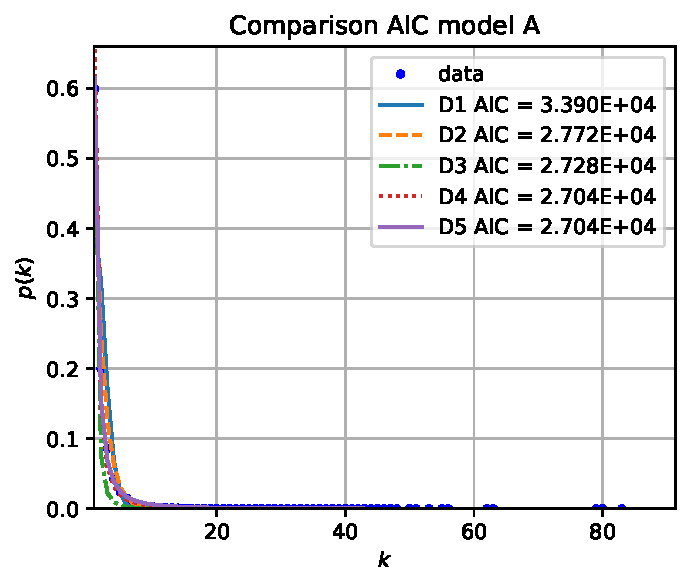
\includegraphics[width=0.5\textwidth]{modelA/all_dd.pdf}
		\caption{Distribution degree for model A}
		\label{fig:all_dd_A}
\end{figure}
%
\begin{figure}[H]
		\centering
		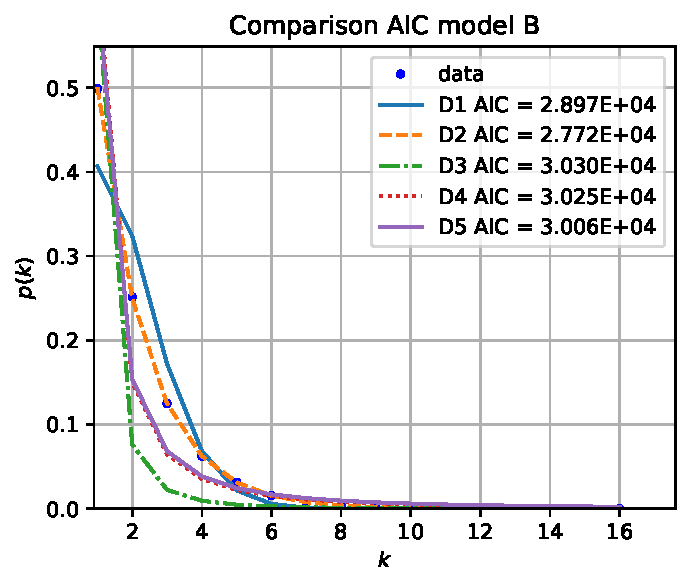
\includegraphics[width=0.5\textwidth]{modelB/all_dd.pdf}
		\caption{Distribution degree for model B}
		\label{fig:all_dd_B}
\end{figure}
%
\begin{figure}[H]
		\centering
		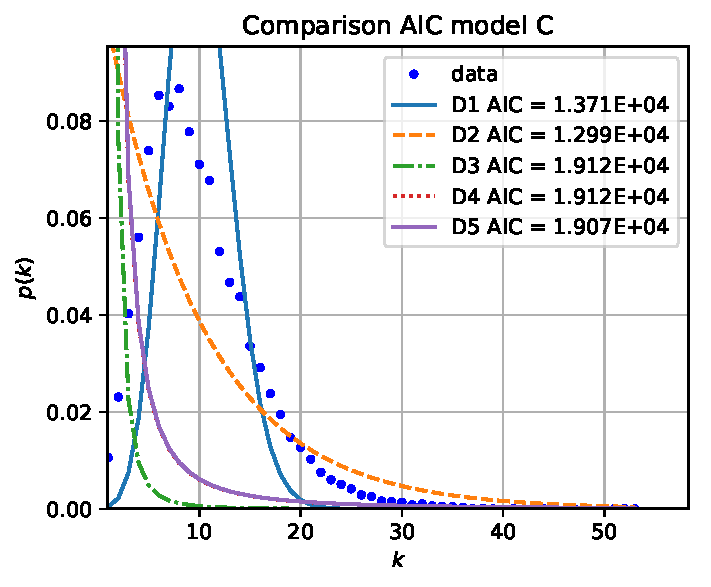
\includegraphics[width=0.5\textwidth]{modelC/all_dd.pdf}
		\caption{Distribution degree for model C}
		\label{fig:all_dd_C}
\end{figure}
%
\begin{figure}[H]
    \centering
		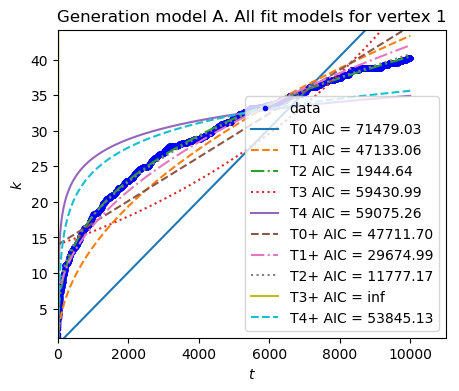
\includegraphics[width=0.5\textwidth]{modelA/all_dt1.png}
		\caption{Degree over time for model A with vertex at $t=1$}
%		\label{fig:all_dd_C}
\end{figure}
%
\begin{figure}[H]
    \centering
		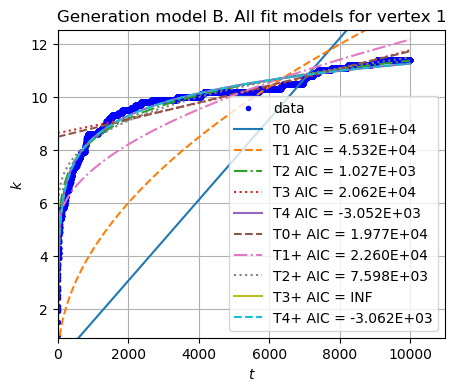
\includegraphics[width=0.5\textwidth]{modelB/all_dt1.png}
		\caption{Degree over time for model B with vertex at $t=1$}
%		\label{fig:all_dd_C}
\end{figure}
%
\begin{figure}[H]
		\centering
		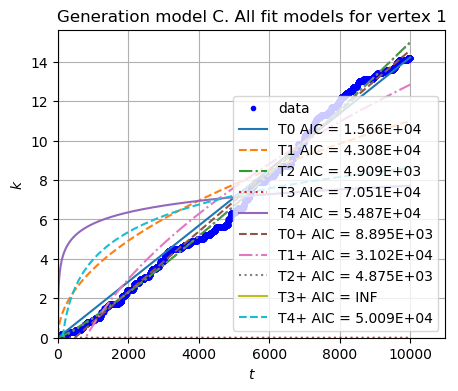
\includegraphics[width=0.5\textwidth]{modelC/all_dt1.png}
		\caption{Degree over time for model C with vertex at $t=1$}
%    \label{fig:all_dd_C}
\end{figure}
%
\begin{figure}[H]
    \centering
		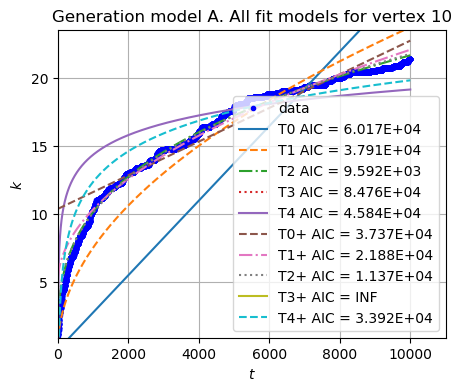
\includegraphics[width=0.5\textwidth]{modelA/all_dt10.png}
		\caption{Degree over time for model A with vertex at $t=10$}
%		\label{fig:all_dd_C}
\end{figure}
%
\begin{figure}[H]
    \centering
		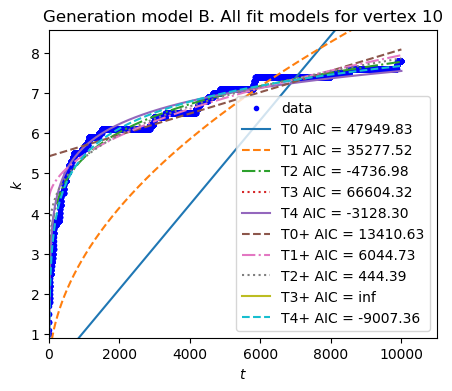
\includegraphics[width=0.5\textwidth]{modelB/all_dt10.png}
		\caption{Degree over time for model B with vertex at $t=10$}
%		\label{fig:all_dd_C}
\end{figure}
%
\begin{figure}[H]
		\centering
		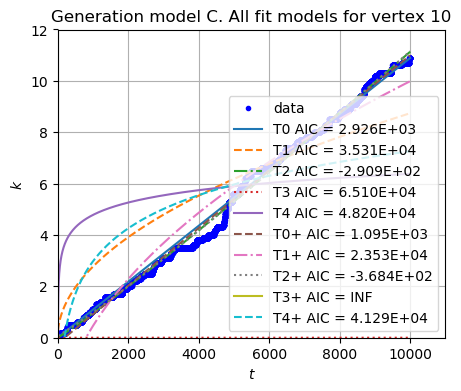
\includegraphics[width=0.5\textwidth]{modelC/all_dt10.png}
		\caption{Degree over time for model C with vertex at $t=10$}
%		\label{fig:all_dd_C}
\end{figure}
%
\begin{figure}[H]
    \centering
		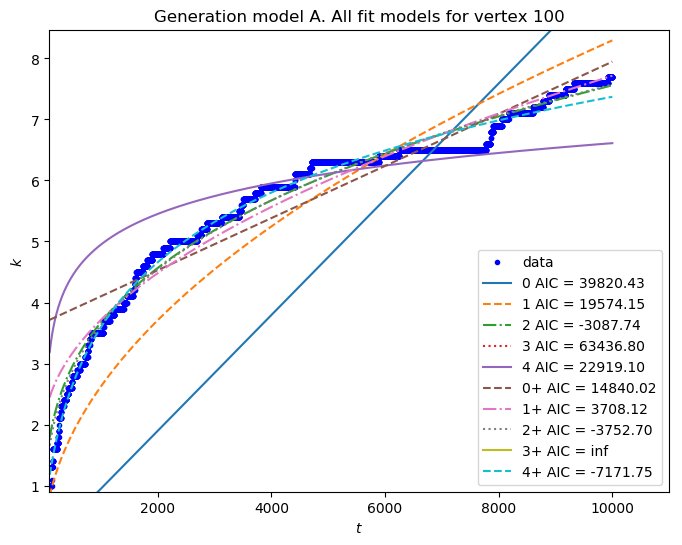
\includegraphics[width=0.5\textwidth]{modelA/all_dt100.png}
		\caption{Degree over time for model A with vertex at $t=100$}
%    \label{fig:all_dd_C}
\end{figure}
%
\begin{figure}[H]
    \centering
		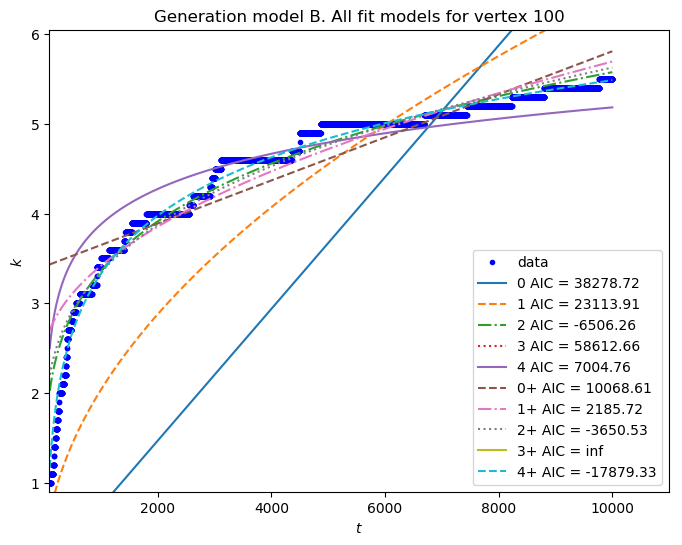
\includegraphics[width=0.5\textwidth]{modelB/all_dt100.png}
		\caption{Degree over time for model B with vertex at $t=100$}
%    \label{fig:all_dd_C}
\end{figure}
%
\begin{figure}[H]
		\centering
		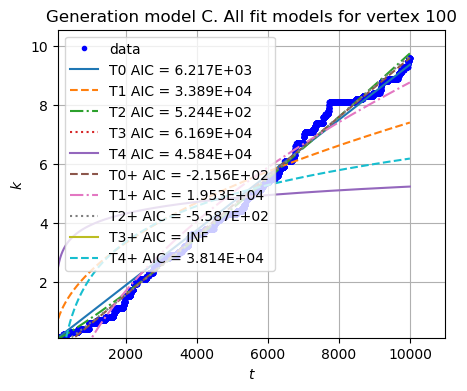
\includegraphics[width=0.5\textwidth]{modelC/all_dt100.png}
		\caption{Degree over time for model C with vertex at $t=100$}
%    \label{fig:all_dd_C}
\end{figure}
%
\begin{figure}[H]
    \centering
		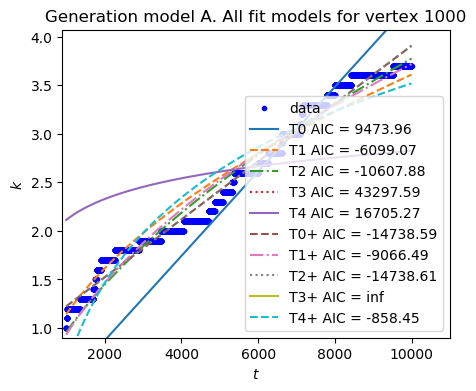
\includegraphics[width=0.5\textwidth]{modelA/all_dt1000.png}
		\caption{Degree over time for model A with vertex at $t=10000$}
%		\label{fig:all_dd_C}
\end{figure}
%
\begin{figure}[H]
    \centering
		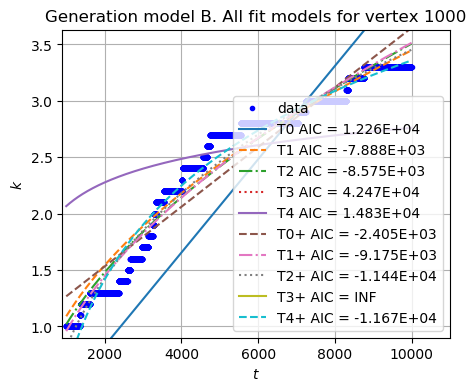
\includegraphics[width=0.5\textwidth]{modelB/all_dt1000.png}
		\caption{Degree over time for model B with vertex at $t=1000$}
%    \label{fig:all_dd_C}
\end{figure}
%
\begin{figure}[H]
		\centering
		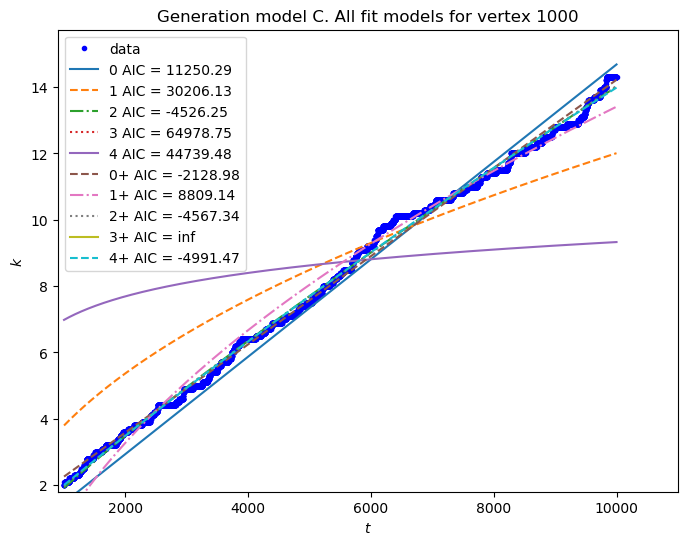
\includegraphics[width=0.5\textwidth]{modelC/all_dt1000.png}
		\caption{Degree over time for model C with vertex at $t=1000$}
		\label{fig:allC_dt1000}
\end{figure}

\end{document}
